\documentclass{article}

\usepackage[english]{babel}
\usepackage[utf8]{inputenc}
\usepackage{amsmath,amssymb}
\usepackage{parskip}
\usepackage{graphicx}

%code
\usepackage{listings}
\usepackage{color}
\usepackage{minted}




% Margins
\usepackage[top=2.5cm, left=3cm, right=3cm, bottom=4.0cm]{geometry}
% Colour table cells
\usepackage[table]{xcolor}

% Get larger line spacing in table
\newcommand{\tablespace}{\\[1.25mm]}
\newcommand\Tstrut{\rule{0pt}{2.6ex}}         % = `top' strut
\newcommand\tstrut{\rule{0pt}{2.0ex}}         % = `top' strut
\newcommand\Bstrut{\rule[-0.9ex]{0pt}{0pt}}   % = `bottom' strut

%%%%%%%%%%%%%%%%%
%     Title     %
%%%%%%%%%%%%%%%%%
\title{CSE344 homework 3}
\author{Ümit Altıntaş \\ 171044005}
\date{\today}

\begin{document}
\maketitle
\section{USAGE}
I got the command line arguments with getopt(), also I have moved the usage print function to the usage.h header for further changing.
\section{VARIABLES}
I have defined main variables as global for easy memory management.
Moved them to the global header file.
\begin{figure}[htbp!]
    \centering
    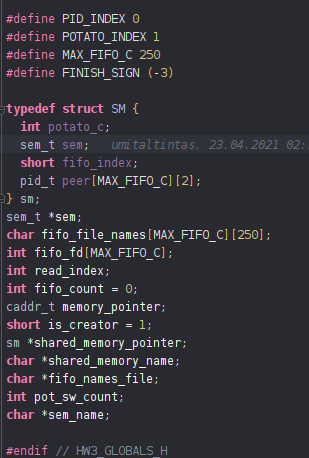
\includegraphics[scale=0.6]{globals.png}
    \caption{globals figure}
    \label{fig:globals}
\end{figure}
\pagebreak

\section{SIGNAL}
I have define a finish function as a signal handler.
\begin{figure}[htbp!]
    \centering
    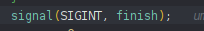
\includegraphics[scale=1]{signal.png}
    \caption{signal figure}
    \label{fig:signal}
\end{figure}

\section{SHARED MEMORY}
First of all I have tried to open file with EXCL  flag so if it is already exist return -1, if it is return -1 I have tried without  EXCL  flag . With this return value have decided who will truncate it  and  create  default values of shared memory.
Lastly all processes write their information to the shared memory.(potato sw number eg.)
\begin{figure}[htbp!]  
    \centering
    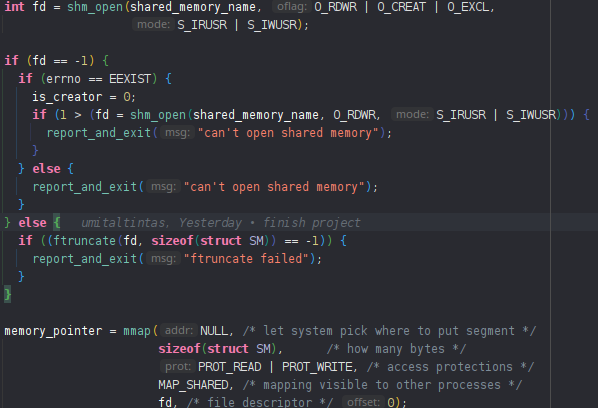
\includegraphics[scale=0.8]{shared.png}
    \caption{shared memory figure}
    \label{fig:shared memory}
\end{figure}
\pagebreak


\section{SEMAPHORE}
I have used to semaphore for synchronization. One for decide who take which fifo file and one for who will write to the shared memory

\begin{figure}[htbp!]  
    \centering
    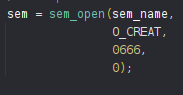
\includegraphics[scale=1]{sem1.png}
    \caption{semaphore figure 1}
    \label{fig:semaphore1}
\end{figure}
This semaphore used for selecting fifo files. it start with 0. after creator process create fifos it post the semaphore. After that they take their fifos respectively. 
For desicion who take which fifo i have used a index insede the shared memory.
\begin{figure}[htbp!]  
    \centering
    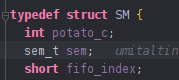
\includegraphics[scale=1]{shrm-fifo-index.png}
    \caption{fifo index figure 2}
    \label{fig:fifo-index}
\end{figure}

\begin{figure}[htbp!]  
    \centering
    
\includegraphics[scale=1]{sem2.png}
    \caption{semaphore figure 2}
    \label{fig:semaphore2}
\end{figure}
This semaphore decides who can change shared memories values.
\pagebreak

\section{FIFO}
After creation fifos they open their fifos as reader and open others as writer. Also fifo file names index and pid indexes(inside the shared memory) are same.
\begin{figure}[htbp!]  
    \centering
    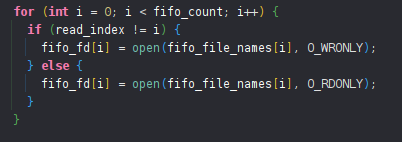
\includegraphics[scale=1]{fifo-open.png}
    \caption{fifo figure 2}
    \label{fig:fifo}
\end{figure}

\section{TRANSFER}
At first they wait for semaphore 2 for getting info's from shared memory. after that if they check their potatoes switch number. if it is not zero select a random fifo and send its potato.
After sending potato post the semaphore and starts reading its fifo. If they read finish signal they they break the loop and call the finish function for memory management, if it is read a valid potato, it wait for semaphore 2 for changing shared memory.
When take permission it decrease the potato switch number and check active potato switch number . If switch number become 0 it decrease  active potato count after that it check active potato count also if it  become 0 sends all fifos a finish signal which is -3 in my case. All of the above is inside a finite loop.
\pagebreak
\begin{minted}[mathescape, linenos]{c}
while (true) {

    // write potato to fifo
    if (-1 == sem_wait(&shared_memory_pointer->sem)) {
      report_and_exit("sem_wait");
    }
    if (shared_memory_pointer->peer[potato_id][POTATO_INDEX]) {
      random_number = select_random_index();
      printf("pid=%d sending potato number %d to %s; %d switches left\n",
             getpid(), shared_memory_pointer->peer[potato_id][PID_INDEX],
             fifo_file_names[random_number],
             shared_memory_pointer->peer[potato_id][POTATO_INDEX] - 1);
      fflush(stdout);
      write(fifo_fd[random_number], &potato_id, sizeof(int));
    }
    if (-1 == sem_post(&shared_memory_pointer->sem)) {
      report_and_exit("sem_post");
    }

    // read potato from fifo
    read(fifo_fd[read_index], &potato_id, sizeof(int));
    if (potato_id == FINISH_SIGN) {
      break;
    } else {

      // update shared memory
      if (-1 == sem_wait(&shared_memory_pointer->sem)) {
        report_and_exit("sem_wait");
      }
      printf("pid=%d receiving potato number %d from %s\n", getpid(),
             shared_memory_pointer->peer[potato_id][PID_INDEX],
             fifo_file_names[read_index]);
      // update switch count
      shared_memory_pointer->peer[potato_id][POTATO_INDEX]--;

      // update potato count
      if (shared_memory_pointer->peer[potato_id][POTATO_INDEX] == 0) {
        printf("pid=%d; potato number %d has cooled down.\n", getpid(),
               shared_memory_pointer->peer[potato_id][PID_INDEX]);
        shared_memory_pointer->potato_c--;
      }
      // handle finish case
      if (shared_memory_pointer->potato_c == 0) {
        send_finish_sign();
        if (-1 == sem_post(&shared_memory_pointer->sem)) {
          report_and_exit("sem_post");
        }
        break;
      }
      if (-1 == sem_post(&shared_memory_pointer->sem)) {
        report_and_exit("sem_post");
\end{minted}
\pagebreak

\section{MEMORY}
Using advantage of the defining main variables as global. I can easyly free and close them with finish function.
    \begin{figure}[htbp!]  
    \centering
    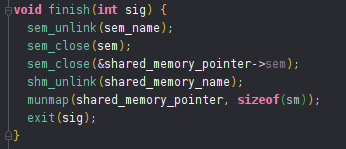
\includegraphics[scale=1]{memory.png}
    \caption{memory figure 2}
    \label{fig:memory}
\end{figure}

\section{FILE STRUCTURE}
-src
--globals.h
--usage.h
--usage.c
--main.c
-makefile
-report.pdf

\end{document}
